% Junior Level 3, Buffer session B1 -- Robot Olympics (unplugged, no computers)
\kcpart{B1}{Robot Olympics}{A clear step rule lets anyone, person or robot, sort a row or solve a maze.}
\lessoninfo{Concepts: step lists and algorithms (R), sorting by a rule (I), maze rule (I), tally and bar graph (R), debugging (R)}{Tools: number cards, the paper maze, crayons, the printables at the end of this plan}{CSTA: 1B-AP-08, 1B-AP-11, 1B-AP-15, 1B-DA-06}

\begin{teachernote}[When to use B1]
Use B1 any time after week 5: after a missed week, before a holiday, on a day the Mac is busy, or when everyone needs a screen break. Everything happens on paper and on the floor. It fits well between weeks 5 and 6 (step rules get children ready to read Python line by line) or before week 9 (planning in steps).
\end{teachernote}

\begin{objectives}
  \item The student can sort a row of number cards by following a written step rule and say how they know the row is sorted. (J3.G2) [J3.B1.1]
  \item The student can solve a paper maze by hand with the \enquote{hand on the right wall} rule and write the moves as a step list a partner can follow. (J3.G2) [J3.B1.2]
  \item The student can find and fix the bug in a sorting rule or a maze step list by acting it out. (J3.G6) [J3.B1.3]
  \item The student can tally the swaps in two sorting races and compare them in a bar graph. (J3.G3) [J3.B1.4]
\end{objectives}

\begin{materials}
  \item Print (from the end of this plan): the number cards (one set per pair, cut apart), the step rule cards, the paper maze (one per child), the race tally and bar graph sheet (one per pair) and the bug cards (one set).
  \item Paper medals: three circles of paper per child, a crayon and a piece of string or tape. Gold, silver and bronze are not needed: every medal says \enquote{Robot Olympian}.
  \item Pencils, crayons and a kitchen timer (for races and Driver/Helper swaps). Prep time: about 10 minutes.
\end{materials}

\needspace{16\baselineskip}
\section{At a glance}
\begin{timeplan}
  \timeslot{0--10}{Warm-up}{The line-up race: children (and toys) hold number cards and line up from smallest to biggest.}
  \timeslot{10--20}{Show me}{A robot needs a rule. Sort four cards together with the neighbor-swap rule and tally each swap.}
  \timeslot{20--33}{Make it}{Sorting races: neighbor-swap and smallest-first with the same six cards. Tally the swaps, then color a bar graph.}
  \timeslot{33--35}{Wiggle break}{Robot relay: walk like a robot, swap places on \enquote{swap!}.}
  \timeslot{35--50}{Make it}{The maze event: solve the paper maze with a hand on the right wall, write the step list, a partner follows it. Bug cards. Free build: design your own event.}
  \timeslot{50--60}{Share}{Medal ceremony with nicknames on the scoreboard. Exit question and reflection.}
\end{timeplan}

\section{Warm-up (0--10 min)}
\begin{unplugged}[The line-up race]
\begin{enumerate}[leftmargin=1.4em,itemsep=1pt]
  \item Hand out number cards from the printable, one per person (toys can hold cards too, so you have at least five). Mix them up.
  \item \enquote{Line up from the smallest number to the biggest. Go!} Time it with the kitchen timer, then check the line together, reading the numbers aloud.
  \item Ask: \enquote{How did you decide where to stand?} Collect the answers: \enquote{I looked at the first digit}, \enquote{I swapped with the person next to me}.
  \item \enquote{People can look at all the cards at once. A robot cannot. It needs a \textbf{step rule}, one small step at a time. Today is the Robot Olympics: every event has a rule, and we follow it like a robot.}
\end{enumerate}
With 1 child: the child places toys holding the cards in a row on the floor; you race the child to sort a second set. With 3 or 4: everyone holds a card, plus a toy or two.
\end{unplugged}

\section{Show me (10--20 min)}
\begin{teacherscript}
\enquote{Here is the \textbf{neighbor-swap rule}. Look at two cards that sit next to each other. If the left one is bigger, swap them, and make a tally mark. Move one place to the right and look again. At the end of the row, start again from the left. When you go all the way along with no swaps, the row is sorted.}
\end{teacherscript}

\begin{analogy}[A referee's rule book]
\enquote{In a race, the referee does not guess who won. They follow the rule book, step by step, the same way every time. A step rule is a rule book for a robot.}
\end{analogy}

\begin{workedexample}[Neighbor-swap with four cards]
Lay four number cards in a row: 305, 47, 812, 120. Read the rule card aloud and do it with a child as the robot; you make the tally marks.
\begin{enumerate}[leftmargin=1.4em,itemsep=1pt]
  \item 305 and 47: the left one is bigger. Swap. Tally 1. Row: 47, 305, 812, 120.
  \item 305 and 812: the left one is smaller. No swap.
  \item 812 and 120: swap. Tally 2. Row: 47, 305, 120, 812. End of the row: start again.
  \item 47 and 305: no swap. 305 and 120: swap. Tally 3. Row: 47, 120, 305, 812. 305 and 812: no swap. Start again.
  \item All the way along with no swaps: sorted! \enquote{Three swaps.}
\end{enumerate}
\enquote{The robot never looked at the whole row. It only looked at two cards at a time, and it still got there.}
\end{workedexample}

\section{Make it (20--33 min)}
\begin{pairroles}[Robot and rule reader]
The \textbf{Driver} is the robot: they move the cards and do only what the rule says. The \textbf{Helper} is the rule reader: they read the next step from the rule card, point at the two cards, and make the tally marks. Swap after each race. With 1 child: the child is the robot first and you read; then swap. With 3: robot, rule reader and referee (checks every step against the rule card), rotating each race. With 4: two pairs racing side by side with the same starting row.
\end{pairroles}

\textbf{Sorting races (about 12 minutes).} Each pair lays out the six race cards in the order on the printable: 650, 120, 990, 47, 333, 509.
\begin{enumerate}[leftmargin=1.4em,itemsep=1pt]
  \item \textbf{Race 1, neighbor-swap.} Follow the neighbor-swap rule. Tally every swap.
  \item \textbf{Race 2, smallest-first.} Put the cards back in the starting order. New rule: find the smallest card in the part that is not sorted yet, and swap it into the first place of that part. Tally every swap.
  \item Color the bar graph on the race sheet: one square for each tally mark. \enquote{Which rule needed fewer swaps?}
\end{enumerate}

\section{Wiggle break (33--35 min)}
Robot relay: everyone walks around stiffly like a robot. When you call \enquote{swap!}, each robot swaps places with the robot nearest to them. When you call \enquote{sorted!}, everyone freezes in a line from shortest to tallest.

\section{Make it (35--50 min)}
\begin{unplugged}[The maze event (about 8 minutes)]
\begin{enumerate}[leftmargin=1.4em,itemsep=1pt]
  \item Hand out the paper maze. \enquote{Here is a rule that solves this maze: put your right hand on the wall and never let go.} Children trace the path with a finger, keeping the right side of the finger against a wall. They will walk into dead ends and come back out: that is fine, the rule still works.
  \item Then they trace the path again with a crayon, this time skipping the dead ends.
  \item Write the step list under the maze, one step per box: an arrow and a number of squares, for example \enquote{up 1}, \enquote{right 2}.
  \item Swap mazes: the partner follows the step list with a finger. Do they reach the finish without crossing a wall?
\end{enumerate}
With 1 child: you follow the child's step list, out loud, and stop if you hit a wall. With 3 or 4: pass the step lists round in a circle.
\end{unplugged}

\begin{bughunt}[Bug cards (about 4 minutes)]
Turn over a bug card. Act it out with the number cards or a finger on the maze. \enquote{What should happen? What happened? Which step is the bug?} Fix it by changing one thing.
\begin{itemize}[leftmargin=1.2em,itemsep=1pt]
  \item \textbf{Bug card 1, The Backwards Robot:} the rule says \enquote{If the left card is \textbf{smaller}, swap them.} The row comes out biggest first. Fix: \enquote{bigger}.
  \item \textbf{Bug card 2, The Stopping Robot:} the rule does not say \enquote{start again from the left}. The robot stops after one trip along the row, and the row is not sorted. Fix: add the step.
  \item \textbf{Bug card 3, The Wall Bumper:} the maze step list says \enquote{up 2} where it should say \enquote{up 1}, so the finger bumps into a wall. Fix: change 2 to 1.
\end{itemize}
\end{bughunt}

\begin{freebuild}[Design an event (about 3 minutes)]
Each child draws their own maze on the blank grid of the maze sheet (a start, a finish, some walls) or invents a new robot event with a rule, such as \enquote{sort the crayons from shortest to longest} or \enquote{line up the toys by size}. A partner tries it at the Share.
\end{freebuild}

\section{Share (50--60 min)}
\begin{safety}[Fair play and nicknames on the scoreboard]
Write a scoreboard with each child's \textbf{nickname} and the events they finished: everyone who finishes an event is an Olympian. \enquote{A scoreboard on a fridge is fine with nicknames. If a game online shows a scoreboard, we use a nickname there too, never our full name, and a grown-up helps.} Then the fair-play rules: kind words for everyone, the same rules for everyone, and credit when a friend's idea helped: \enquote{Priya's maze idea gave me my maze.}
\end{safety}

\begin{teacherscript}
Hand each child a paper medal with their nickname. Children try one partner's own maze or event. \enquote{Did the rule work for someone else? That is the test of a good step list.}
\end{teacherscript}

\begin{formativecheck}[Exit question]
\textbf{Look for:} the robot follows the rule and does not skip ahead; tally marks in groups; a step list a partner can follow; one bug found by acting it out.

\textbf{Ask:} show two cards, 509 and 333, in that order. \enquote{The neighbor-swap rule is looking at these two. What does the robot do?}
\textbf{Answer:} swap them, because the left card (509) is bigger, and make a tally mark.
\end{formativecheck}

\begin{reflection}
Ask: \enquote{Which event did you like best: sorting, the maze or the bug cards?} and \enquote{Which rule was faster, and how does the bar graph show it?} Children draw a smiley on their medal next to their favorite event.
\end{reflection}

\section{Notes for the teacher}
\begin{commonmistakes}
  \item \textbf{Skipping ahead.} A child sees where 47 belongs and moves it at once. Praise the thinking, then: \enquote{A robot can only look at two cards. Let us follow the rule.}
  \item \textbf{Comparing by the first digit only.} 990 and 120 are easy, but 47 and 305 are not: 47 is smaller because it has only two digits. Read the numbers aloud (\enquote{forty-seven}, \enquote{three hundred five}).
  \item \textbf{Forgetting to start again.} One trip along the row is not always enough. The rule ends only after a trip with no swaps.
  \item \textbf{Right hand, wrong wall.} In the maze, the right hand stays on the wall to the right of the way you face. Turning the paper as you go helps.
  \item \textbf{Step lists with turns.} Children may write \enquote{turn left}. Arrows that say which way on the page (up, down, left, right) are easier to follow on paper.
\end{commonmistakes}

\begin{differentiation}
\supportpath Race with four cards, all two-digit numbers (for example 47, 12, 90, 33). In the maze, trace with a finger only and skip the written step list; say the steps aloud instead.
\extensionpath Race with eight cards, including 333 and 330. Write the neighbor-swap rule as a numbered step list in your own words, with a \enquote{repeat until} step, like a Scratch \enquote{repeat until} block.
\end{differentiation}

\begin{stretchchallenge}[The shortest path]
In the maze, which path has the fewest steps? Count the squares. Does the right-hand rule find the shortest path, or only a path?
\end{stretchchallenge}

\begin{teachernote}[If you are short on time]
Do the line-up race and one sorting race (neighbor-swap). Do the maze without the written step list. Use bug card 1 only. Keep the wiggle break and the medals.
\end{teachernote}

\begin{teachernote}[Answers]
\textbf{Race 1, neighbor-swap} (650, 120, 990, 47, 333, 509): 8 swaps. \textbf{Race 2, smallest-first}: 4 swaps (47 to the front; 120 is already in place; then 333, 509 and 650 each move with one swap). Sorted row: 47, 120, 333, 509, 650, 990. Children may count one more or one fewer if they slip; the bar graph should still show that smallest-first used fewer swaps (but it needed more looking).
\textbf{Paper maze}, from START (bottom left): up 1, right 1, down 1, right 2, up 1, left 1, up 1, right 2, up 1, left 1, up 1, right 1, up 1 to FINISH. The dead ends are at the bottom right and on the left side; the right-hand rule walks into the bottom-right one and back out.
\textbf{Bug cards:} 1. change \enquote{smaller} to \enquote{bigger}; 2. add \enquote{at the end of the row, start again from the left, until a trip has no swaps}; 3. change \enquote{up 2} to \enquote{up 1}.
\end{teachernote}

\section{Printables}
\subsection*{Printable 1: number cards (cut apart, one set per pair)}
The first six are the race cards. The last four are for the warm-up and the worked example.
\begin{center}
\Huge\renewcommand{\arraystretch}{2.2}
\begin{tabular}{|*{5}{>{\centering\arraybackslash}p{2.6cm}|}}
\hline
650 & 120 & 990 & 47 & 333\\ \hline
509 & 305 & 812 & 76 & 201\\ \hline
\end{tabular}
\end{center}

\subsection*{Printable 2: step rule cards}
\begin{center}
\renewcommand{\arraystretch}{1.4}
\begin{tabular}{|p{7cm}|p{7cm}|}
\hline
\textbf{Neighbor-swap rule} & \textbf{Smallest-first rule}\\
1. Look at the first two cards. & 1. Look at every card that is not sorted yet.\\
2. If the left card is bigger, swap them. Make a tally mark. & 2. Find the smallest one.\\
3. Move one place to the right. Look at the next two. & 3. Swap it into the first place that is not sorted yet. Make a tally mark (no mark if it is already there).\\
4. At the end of the row, start again from the left. & 4. That place is now sorted. Go back to step 1.\\
5. Stop when a whole trip has no swaps. & 5. Stop when every place is sorted.\\ \hline
\end{tabular}
\end{center}

\subsection*{Printable 3: race tally and bar graph (one per pair)}
Starting row: \textbf{650, 120, 990, 47, 333, 509}.
\begin{center}
\Large\renewcommand{\arraystretch}{1.6}
\begin{tabular}{|p{5cm}|p{7cm}|}
\hline
Race 1: neighbor-swap & \\ \hline
Race 2: smallest-first & \\ \hline
\end{tabular}
\end{center}
\begin{center}
%% alt: An empty bar graph with two columns labeled neighbor-swap and smallest-first, and squares numbered 1 to 10 going up.
\begin{tikzpicture}[x=1cm,y=0.8cm]
  \foreach \c/\name in {0/neighbor-swap,1/smallest-first} {
    \foreach \r in {0,...,9}
      \draw[kcgray!80!black,line width=0.8pt] (1.2+\c*4,\r) rectangle ++(2.4,1);
    \node[font=\large\bfseries] at (2.4+\c*4,-0.6) {\name};
  }
  \foreach \r in {1,...,10}
    \node[font=\large] at (0.6,\r-0.5) {\r};
\end{tikzpicture}
\end{center}

\clearpage
\subsection*{Printable 4: the paper maze (one per child)}
Start at the bottom left. Keep your right hand on the wall. Reach the finish at the top right.
\begin{center}
%% alt: A square maze of 5 by 5 squares with thick walls. The entrance labeled START is at the bottom of the bottom-left square and the exit labeled FINISH is at the top of the top-right square. There are dead ends on the left side and in the bottom-right corner.
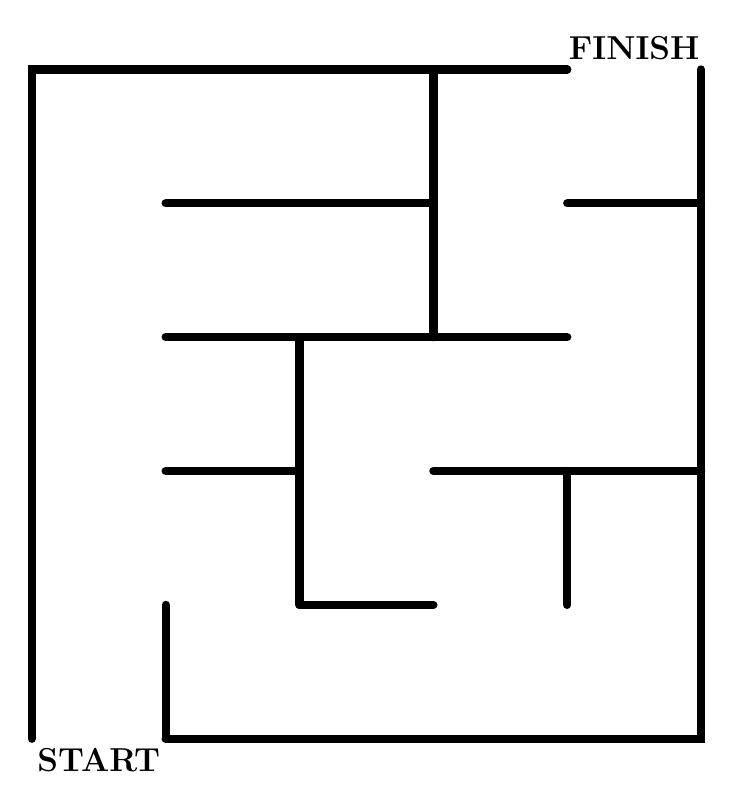
\begin{tikzpicture}[x=1.7cm,y=1.7cm,wall/.style={line width=3pt,line cap=round}]
  % outer walls, with a gap for the start (bottom left) and the finish (top right)
  \draw[wall] (1,0) -- (5,0) -- (5,5);
  \draw[wall] (4,5) -- (0,5) -- (0,0);
  % inner walls (vertical)
  \draw[wall] (1,0) -- (1,1);
  \draw[wall] (2,1) -- (2,3);
  \draw[wall] (4,1) -- (4,2);
  \draw[wall] (3,3) -- (3,5);
  % inner walls (horizontal)
  \draw[wall] (1,2) -- (2,2);
  \draw[wall] (1,3) -- (3,3);
  \draw[wall] (1,4) -- (2,4);
  \draw[wall] (2,1) -- (3,1);
  \draw[wall] (2,4) -- (3,4);
  \draw[wall] (3,2) -- (5,2);
  \draw[wall] (3,3) -- (4,3);
  \draw[wall] (4,4) -- (5,4);
  \node[font=\large\bfseries,below] at (0.5,0) {START};
  \node[font=\large\bfseries,above] at (4.5,5) {FINISH};
\end{tikzpicture}
\end{center}
My step list (one step in each box, for example \enquote{up 1}):
\begin{center}
\renewcommand{\arraystretch}{2.2}
\begin{tabular}{|*{7}{p{1.6cm}|}}
\hline
 & & & & & & \\ \hline
 & & & & & & \\ \hline
\end{tabular}
\end{center}
My own maze (draw walls on the dotted grid):
\begin{center}
%% alt: An empty 5 by 5 grid of dotted lines for drawing a maze.
\begin{tikzpicture}[x=1.2cm,y=1.2cm]
  \draw[kcgray,dotted,line width=1pt] (0,0) grid (5,5);
\end{tikzpicture}
\end{center}

\subsection*{Printable 5: bug cards (cut apart)}
\begin{enumerate}[leftmargin=1.6em,itemsep=4pt]
  \item \textbf{The Backwards Robot.} Goal: smallest to biggest. Rule: \enquote{If the left card is smaller, swap them.} What happened: the row came out biggest first.
  \item \textbf{The Stopping Robot.} Goal: smallest to biggest. Rule: 1. Look at the first two cards. 2. If the left card is bigger, swap them. 3. Move one place to the right. 4. Stop at the end of the row. What happened: with 650, 120, 990, 47, 333, 509 the row ended as 120, 650, 47, 333, 509, 990. Not sorted!
  \item \textbf{The Wall Bumper.} Goal: reach the finish of the paper maze. Steps: up 1, right 1, down 1, right 2, up 2, \ldots{} What happened: the finger bumped into a wall.
\end{enumerate}
